\chapter{Evaluation}
\label{chapt:evaluation}

This chapter describes the evaluation of the two different implementations of the system architecture. In the first architecture, more than one memcached instances at layer 2 were introduced, as figure~\ref{fig:system_architecture} shows. In the second, more than one Social Network engines were introduced at layer 1.

In order to measure the response time (RT) the Apache JMeter application~\cite{jmeter_url} is used. The Apache JMeter is an open source benchmark designed to test functional behaviour and  measure performance, targeting web applications. Notably, the RT measured by JMeter may not be the real one, because the JMeter measures the elapsed time from just before sending the request to just after the last response from the server has been received. As a result, the time to render the web page to the client web browser and the execution time of JavaScript code is not measured. Because those two time intervals are client limited and depend on client performance and on which web browser is used, they are excluded from the following performance test benches. For the next experiments, a specific web page will be used. This page does not use any AJAX call, in order to not misguide the results. Therefore, the RT measures the time from just before JMeter sends the request to just after the last response is received. During this measured time interval, the Social Network engine performs the following actions:
\begin{enumerate}[I]
\item The Social Network engine sends a request to CDO Client for the application execution model.
\item The CDO Client forwards this request to CDO Server.
\item Afterwards CDO Server queries the mysql repository of application models and executions, and finally gets the executions results.
\item CDO Server forwards the results through the CDO Client to the Social Network Engine.
\item Finally, the Social Network engine sends queries to the Social Network DB in order to get all the necessary Social features for this application page
\end{enumerate}

\section{Improving Performance with memcached}
\label{sec:eval_memcache}
By adding a memcached node at the system architecture, the Social Network Engine first asks the memcached node if it has the tuples that the SN Engine needs. So the steps(\emph{I} to \emph{V}), mentioned previously, are not necessary if the memcached node has cached the values that the Social Network Engine needs. The loop through CDO CIient - CDO Server and the repositories is bypassed. 

For the following experiments all the memcached nodes are warm up and have cached all the needed CDO and Social entities information. Furthermore the CDO server has been warm up after a fresh restart. As the table~\ref{tab:num_of_queries} shows
the starting process of the CDO server produces 1938 queries to MySQL database. The \emph{fresh query} for an application model (both social information and executions) produces 15182 queries to MySQL database. The CDO server caches the results, so a second query for this application model produces 251 queries, which the most of them are the queries for the social information of the application. Introducing memcached, if the request for the application model is cached, the queries to database are lowering to 147.  

The test performed with the following loads: (L1) ten users requests \emph{two} applications, (L2) ten users requests \emph{four} applications and (L3) ten users requests \emph{eight} applications. All three Loads run consecutively one hundred times each. Those Loads request applications, which have ten execution rows pulled from the repository of applications models and executions, and about one hundred queries to the Social Network DB. In this experiment we kept constant the following components of the system: the Elgg front-end Apache2 server, the Social network BD, and the CDO server - client communication but increased the number of memcached nodes.
The figure~\ref{fig:rtavg} shows the  average, minimum and maximum response time (RT) in milliseconds with the following system configuration: (C1) no memcached node, (C2) one memcached node and (C3) two memcached nodes.

\begin{figure}[h]
	\caption{The average response time for all configurations.}
	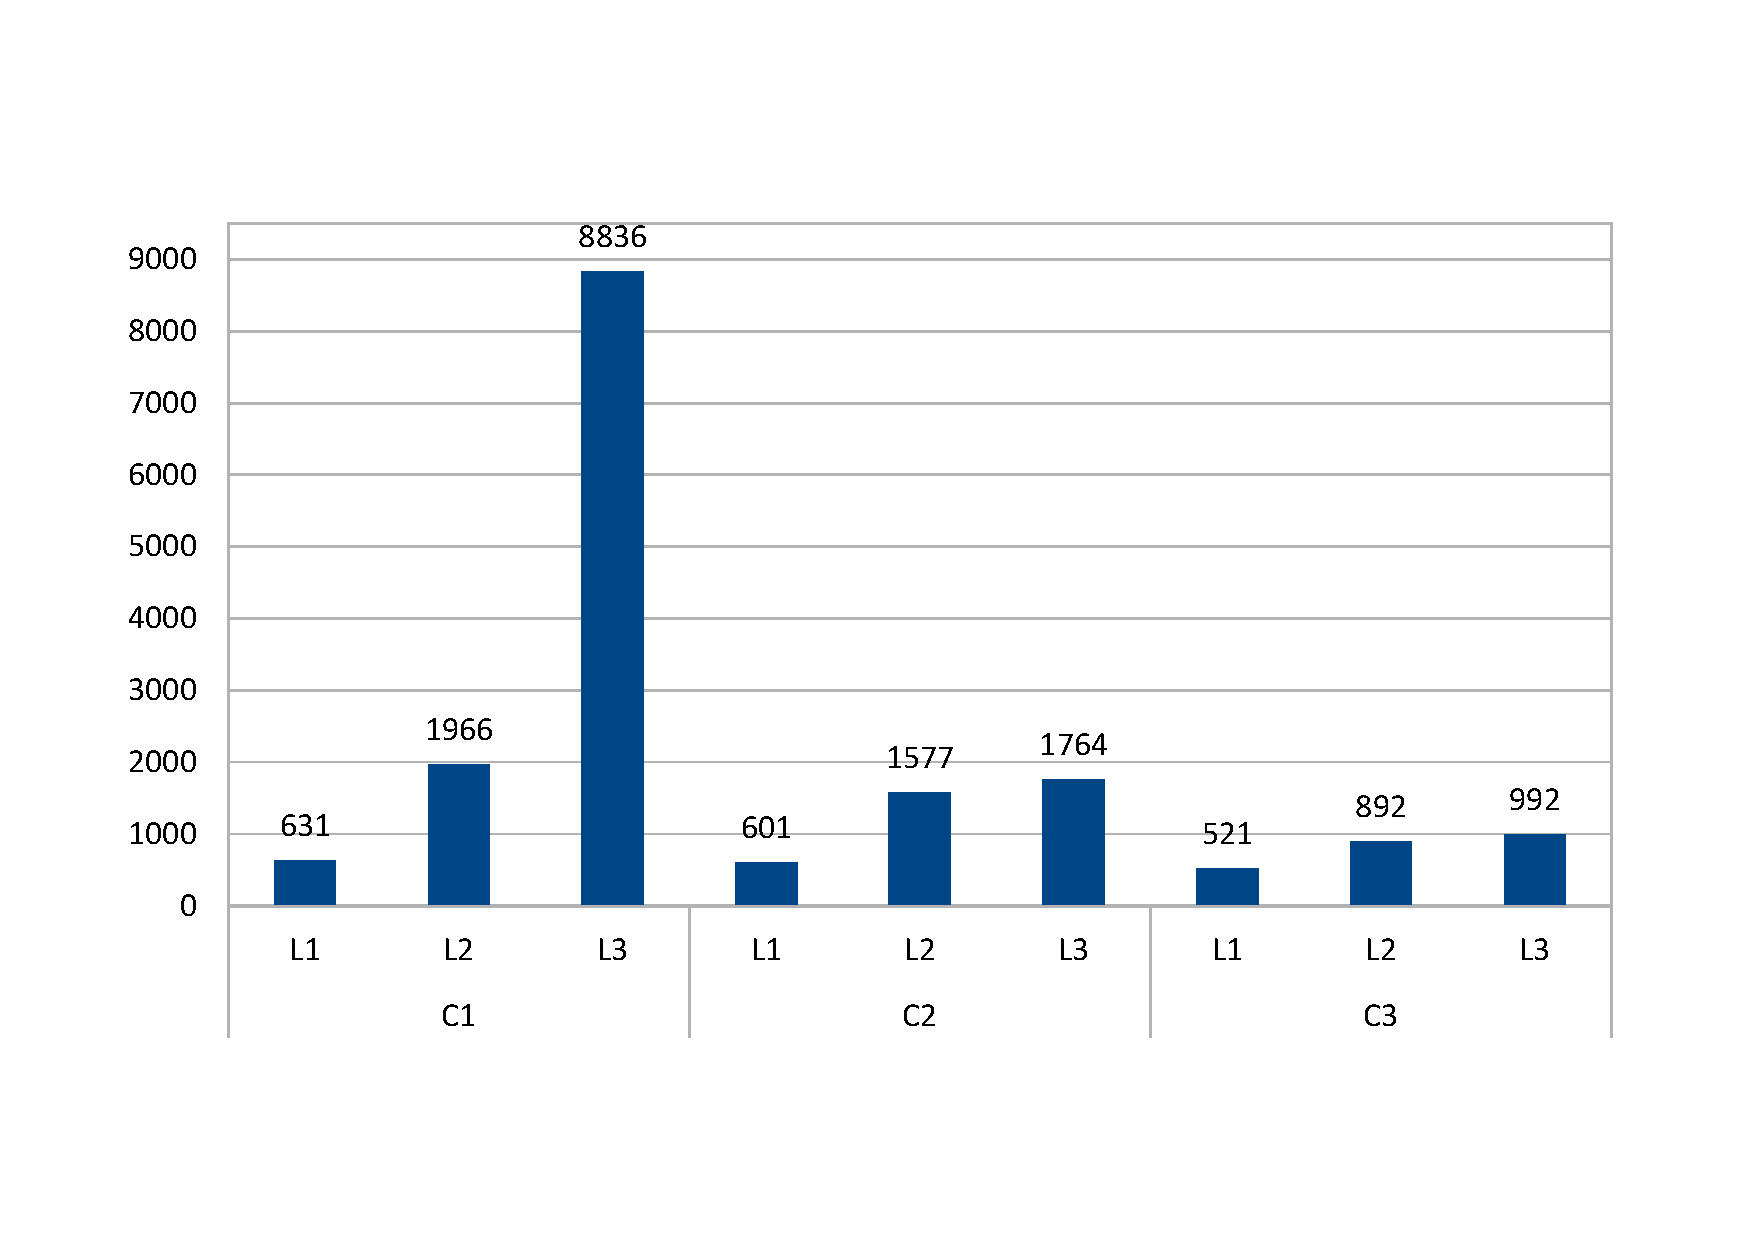
\includegraphics[width=0.6\textwidth,natwidth=200,natheight=150]{./fig/RTavg.pdf}
	\centering
	\label{fig:rtavg}
\end{figure}

As we going from C1 to C3 and specifically for L(oad) 3, the RT is reduced by 80,4\% at C2 and by 88,78\% at C3. As the figure~\ref{fig:rtavg} shows, at the first configuration C1, the L3 takes 8836 ms, an RT which is definitely prohibitive for web applications. Introducing more memcached nodes at C2 and C3 the RT is decreased dramatically at 1764 ms at L2 and at 992 ms at L3. Going from C1 to C2, the 80,4\% reduction of RT is due to the introduction of memcached node and bypassed the steps I - V. Going from C2 to C3, the 43,77\% reduction of RT is due to adding more memcached nodes, resulting to more cpu cores  introduced to the architecture.

\begin{table}[]
\centering
\caption{Number of Queries to Social Network and CDO server Databases.}
\label{tab:num_of_queries}
\begin{tabular}{ll}
State        & \# of Queries \\
Fresh start  & 1938          \\
Fresh Query  & 15182         \\
Cached Query from CDO & 251           \\
Cached Query from Memcached & 147  
\end{tabular}
\end{table} 

\begin{figure}[h]
	\caption{The average CPU utilization for all components.}
	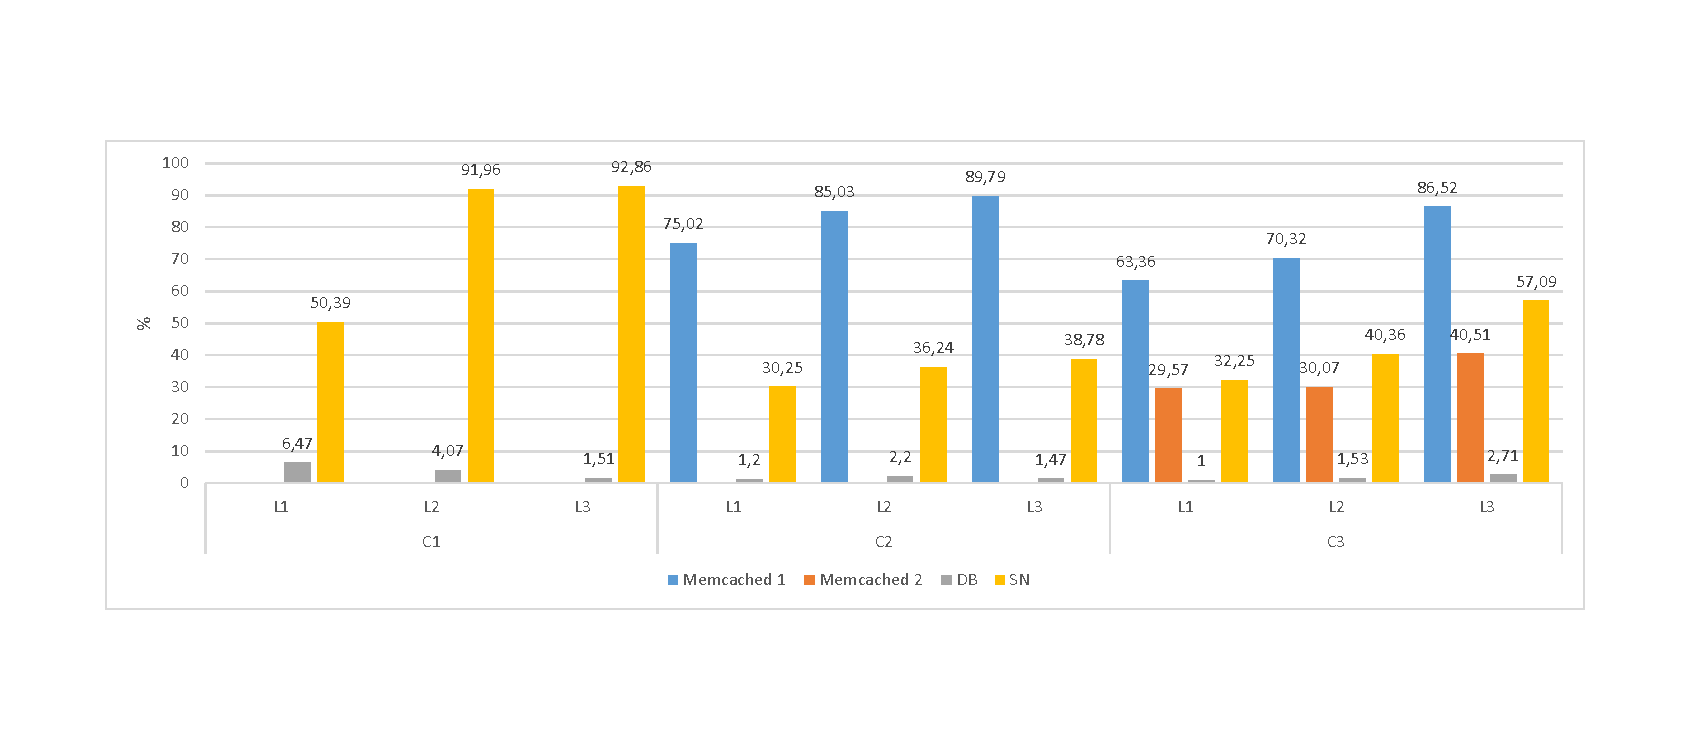
\includegraphics[width=1\textwidth,natwidth=200,natheight=150]{./fig/UsageAVG.pdf}
	\centering
	\label{fig:cpuavg}
\end{figure}

Furthermore, the CPU utilization is measured using the sysstat tool~\cite{sysstat_url}. We measured the CPU utilization for all the VMs running the experiment. The information about the VM resources is listed in the table~\ref{table:vms_resources}. The Social Network Engine and the CDO Client were running at t1.micro instance. The mysql (repositories) and the CDO Server were running at m1.xlarge. The average CPU utilization is shown in the figure~\ref{fig:cpuavg}. At the simple configuration C1, even in small loads such as L1, the SN Engine reached 50,39\% CPU utilization. In the medium load L2 and big load L3 the SN Engine is kneeled down to 91,96\% and 92,86\%. This big consumption of CPU was due to all the initialization that Elgg Social Network Engine has to do for each request and due to CDO Server queries.

Moving from configuration C1 to C2, the CPU consumption went to memcached node. Thus, the Social Network engine was de-congested and the RT improved. However, for the big load L3 the memcached node reached 89,79\%. To solve memcached CPU overhead, one more memcached node was added at configuration C3. This second memcached node shared the CPU overhead with the first memcached node and the RT improved furthermore. For all three loads at C3, the first memcached node has more CPU utilization from the second by an approximately factor of 2,2. This difference between the two memcached nodes appeared due to the first node storing more popular key-value pairs than the other.

\begin{table}[]
\label{table:vms_resources}
\centering
\caption{VM resources}
\label{my-label}
\begin{tabular}{|l|l|}
\hline
 Component &  VM type \\ \hline
 SN engine, CDO client &  t1.micro \\ \hline
 memcached &  t1.micro \\ \hline
 repositories, CDO Server &  m1.xlarge \\ \hline
 jmeter &  m1.large \\ \hline
\end{tabular}
\end{table}

\section{Improving Performance with engine}
This section evaluates the horizontal scale of Social Network engine as described in~\ref{sec:engine_scale}. A memcached node was living between the Social Networking Engines and the back end system. The VM resources are kept the same in the previous experiment, shown in the table~\ref{table:vms_resources}. One more Social Networking Engine instance was added with the same type as former SN Engine. The load from one SN Engine is now distributed to two SN Engines instances. So, the response time improved, as shown in the figure~\ref{fig:rt2SN} for the Load 3 compared to the previous test-bench. 

\begin{figure}[h]
	\caption{The Response time for two Social Network Engines.}
	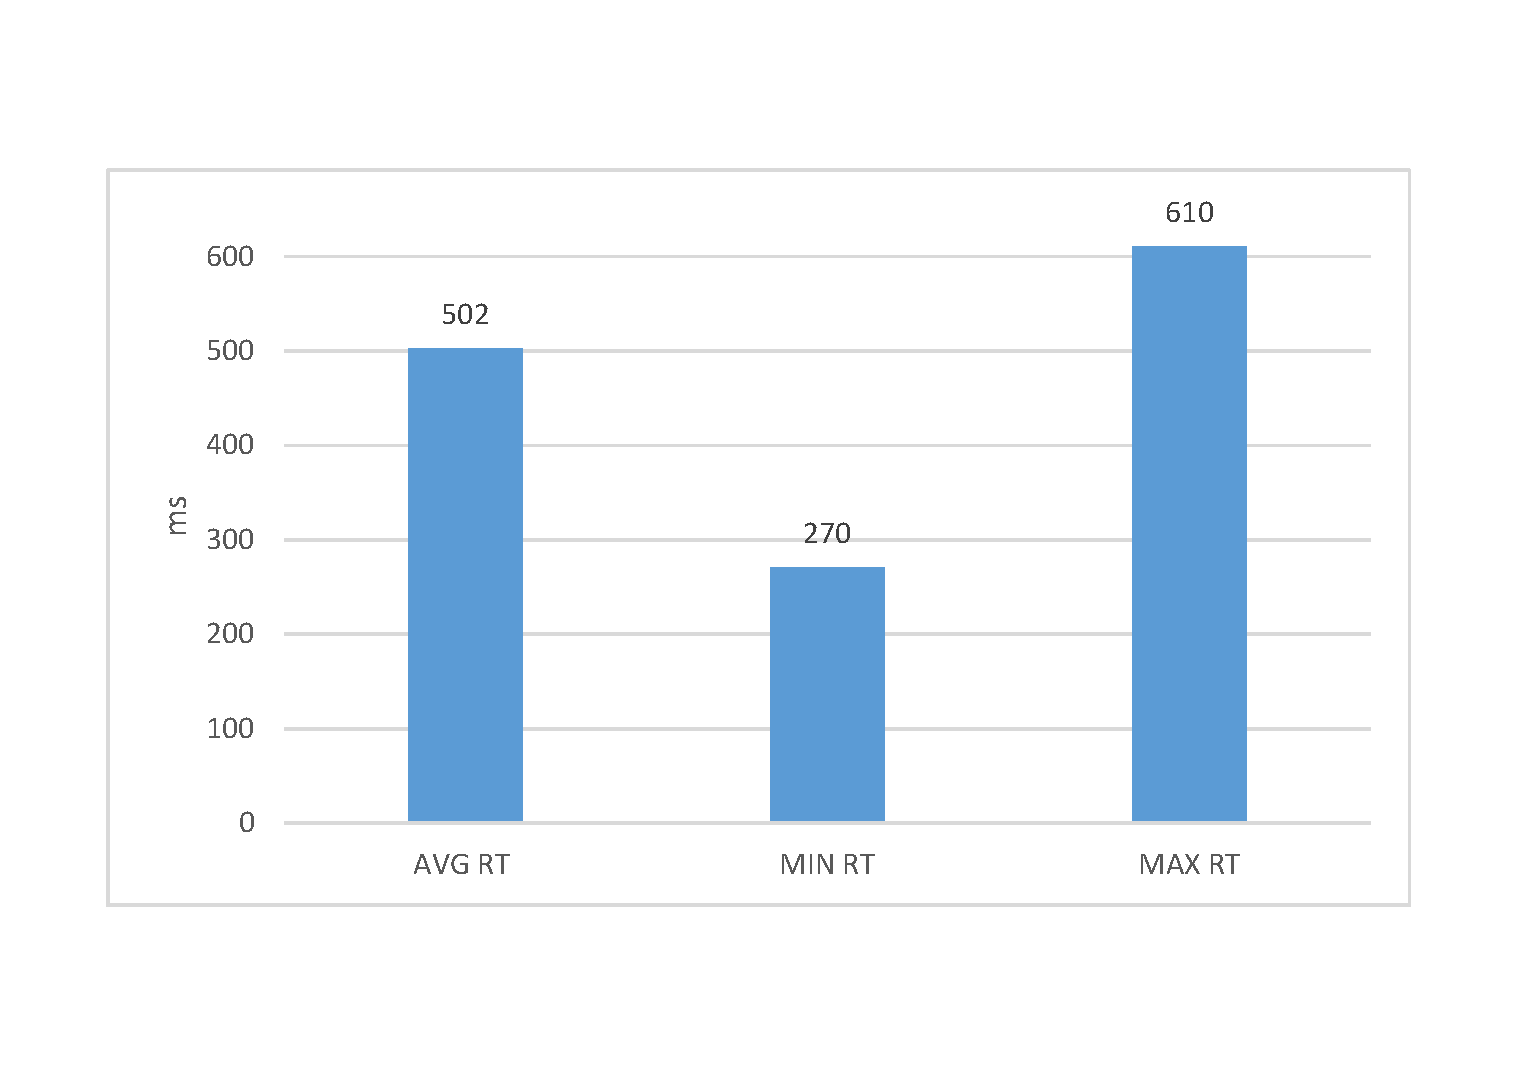
\includegraphics[width=1\textwidth,natwidth=200,natheight=150]{./fig/RT2SN.pdf}
	\centering
	\label{fig:rt2SN}
\end{figure}

The CPU utilization to SN Engines decreased as shown in the figure~\ref{fig:cpu2SNavg}. This reduction is due to the requests being distributed to two instances instead of only one. The CPU utilization of the memcached node increased, but this can be solved by introducing more memcached nodes as the previous section describes. 

\begin{figure}[h]
	\caption{The CPU utilization for two Social Network Engines.}
	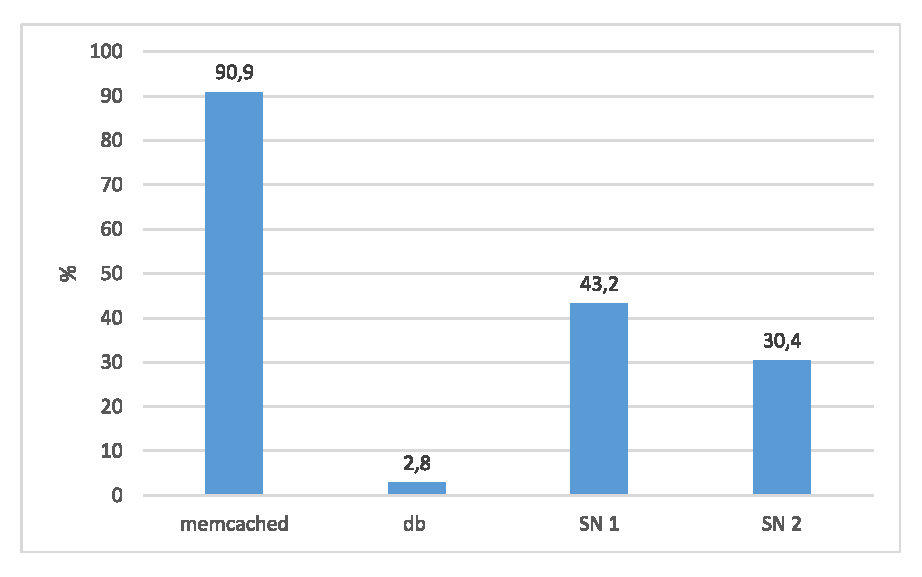
\includegraphics[width=1\textwidth,natwidth=200,natheight=150]{./fig/Usage2SN.pdf}
	\centering
	\label{fig:cpu2SNavg}
\end{figure}

\section{Evaluation of NLP classification}
\label{sec:nlp_evaluation}
This section evaluates the Natural Language Processing Tool as described in section~\ref{sec:natural_implementation} for the first training set. This set had five different classes or, according to StackOverflow dialect, five tags, as described in~\ref{sec:natural_implementation} and shown in table~\ref{table:nlp_eval}. For the testing set, thirty questions from StackOverflow were used per class. Those questions were different from the training set and had the highest activity during that specific time period. Each row at table~\ref{table:nlp_eval} shows a class as classified by StackOverflow users, and each column shows how our classifier classifies the question. For example, twenty one questions about \emph{reliability} were classified correctly, but eight were wrongly classified as \emph{optimization} and one was wrongly classified as \emph{performance}. The misclassification was not an error of our classifier but some questions from the testing set were either wrongly classified by the StackOverflow users or had more than one tags. For example, one question that was wrongly classified as \emph{performance} instead of \emph{reliability} was: ``can somebody explain me how to handle errors. my code is: \ldots''. The above question is out of the scope of reliability and even though the user tagged it as a reliability question, it was downvoted and marked as ``very low quality'' from the StackOverflow community.

Another example showing that the classifier is not misclassifying is the following question:
``I want to perform some data manipulation tasks and analysis in spark and want to \textbf{optimize} the run times. 
here is the problem: \ldots ''. 
This question was marked by the user with both scalability and optimization tags. Even though this question is retrieved with the scalability tag and in the table it is shown as a wrong classification, after examining this question, one can realize that the \emph{scalability} tag was wrongly added by the user and only the \emph{optimization} tag should be placed.

This shows that our tool can further be used by StackOverflow to mark new questions that are wrongly tagged or misguided. There is a trend among StackOverflow users to add as many tags as they can in order to attract the attention of other users, increase the views of their question and finally get their answers.  

\begin{table}[]
\centering
\caption{NLP Evaluation of Classification}
\label{table:nlp_eval}
\begin{tabular}{|l|c|c|c|c|c|}
\hline
class / class & \multicolumn{1}{l|}{reliability} & \multicolumn{1}{l|}{design} & \multicolumn{1}{l|}{optimazation} & \multicolumn{1}{l|}{performance} & \multicolumn{1}{l|}{scalability} \\ \hline
reliability   & \textbf{21}                    & 0                           & 8                                 & 1                                & 0                                \\ \hline
design        & 2                                & \textbf{15}               & 8                                 & 3                                & 2                                \\ \hline
optimazation  & 2                                & 3                           & \textbf{15}                     & 9                                & 1                                \\ \hline
performance   & 2                                & 1                           & 17                                & \textbf{9}                     & 1                                \\ \hline
scalability   & 10                               & 6                           & 3                                 & 3                                & \textbf{8}                     \\ \hline
\end{tabular}
\end{table}
